\subsection{Diagnostic Evidence and Architecture-Aware Inspection}
\label{sec:shap_module_results}

The diagnostic evidence was first evaluated at the telemetry level to determine whether the TreeSHAP-based hierarchy preserved attribution information and whether the identified features were relevant to model predictions. Across the 3,602 labelled anomalous test windows, aggregation from statistical features to telemetry channels, uORB topics, and functional subsystems preserved the total attribution magnitude, with a maximum absolute conservation error of $7.11\times10^{-15}$. This confirms the numerical consistency of the hierarchical aggregation, although conservation alone does not imply that a high-ranked feature or channel is the physical source of the anomaly.

Prediction relevance was further examined through attribution-guided masking. Features were ranked using validation-derived TreeSHAP importance and then masked on the test set using training-derived replacement values. As shown in Figure~\ref{fig:shap_module_evidence}(a), masking the SHAP-ranked features caused a consistently larger decrease in Macro-F1 than masking an equal number of randomly selected features. The performance drop increased from 0.0409 when masking the top 10 features to 0.2683 for the top 100 features. The corresponding paired SHAP-minus-random differences were 0.0404 (95\% CI [0.0102, 0.0713]) and 0.2646 (95\% CI [0.2052, 0.3300]), respectively. The same trend was observed when the selected feature blocks were replaced by sampled training examples rather than feature-wise medians. These results indicate that the attribution ranking concentrates prediction-relevant information rather than merely reflecting arbitrary feature ordering.

The agreement between highly ranked telemetry channels and the annotated fault domains was less uniform. Under the document-derived semantic mapping, overall Consistency@1 was $0.2500\pm0.0056$, compared with a random baseline of 0.1707. The agreement varied across fault domains, indicating that predictive relevance and semantic fault-domain correspondence should be treated as complementary rather than equivalent properties. The masking results therefore support the relevance of the identified evidence to the classifier, but do not establish a causal relationship between the highlighted channels and the underlying physical fault.

Topic-level evidence was subsequently propagated through the commit-specific PX4 uORB dependency graph to obtain architecture-aware software inspection candidates. After conservative source-path filtering, the graph retained 145 topic--module relations covering 36 PX4 modules while preserving all evaluated telemetry topics. Under producer-oriented propagation, the highest-ranked candidates were \path{src/modules/mavlink}, \path{src/modules/ekf2}, \path{src/modules/sensors}, \path{src/modules/vtol_att_control}, and \path{src/modules/position_estimator_inav}, with normalized SHAP shares of 0.2572, 0.2318, 0.1243, 0.0811, and 0.0708, respectively. Figure~\ref{fig:shap_module_evidence}(b) summarizes these candidate scores.

The architecture-aware ranking should be interpreted as an inspection aid rather than direct fault localization. Multiple modules may publish the same uORB topic, and static publisher--subscriber relations do not establish execution-time causality. In addition, only anomalies detected by Stage 1 can contribute evidence in a deployed pipeline. Under the matching-commit detector-gated analysis, the mean Stage 1 recall was $0.6728\pm0.0248$, which bounds the fraction of labelled real-flight anomalies that can reach the downstream evidence and module-ranking stages. The resulting software-module scores therefore represent telemetry-driven inspection priorities conditioned on successful anomaly detection, not verified source-level root causes.

\begin{figure}[H]
    \centering
    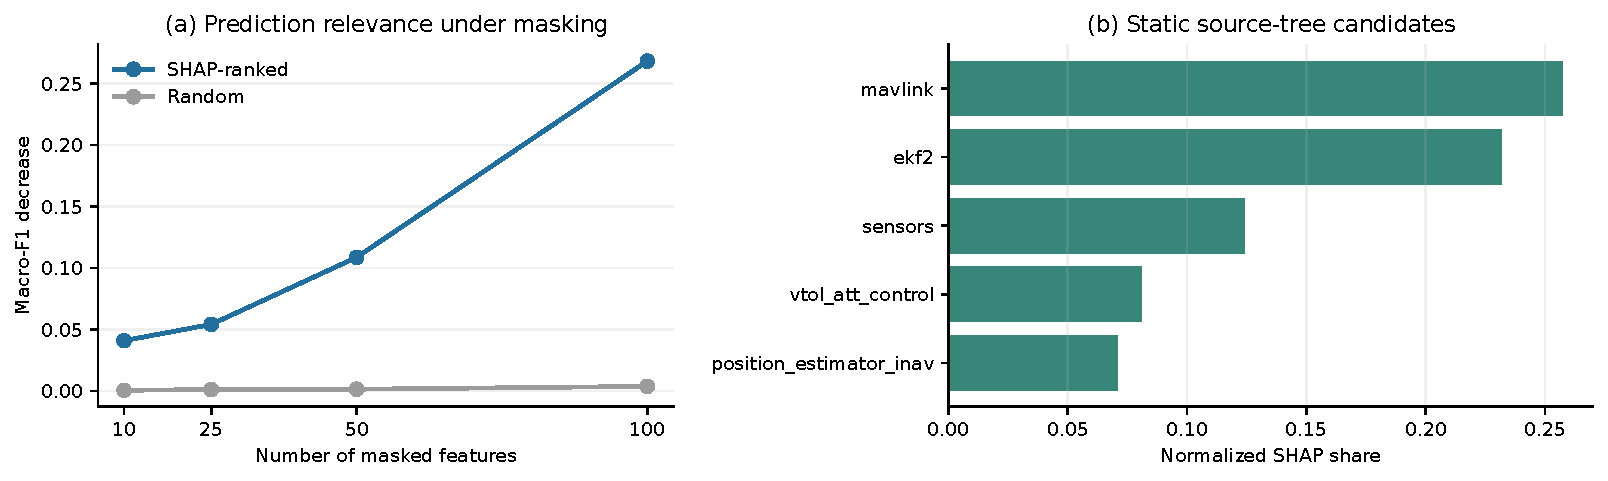
\includegraphics[width=\textwidth]{figures/figure_2_shap_evidence_module_ranking.pdf}
    \caption{Prediction-relevant evidence and architecture-aware candidates. (a) Mean Macro-F1 decrease after masking validation-ranked SHAP features or equal-size random subsets. (b) Filtered producer-only source-tree candidates from matching-commit anomalous test windows; bars show mean normalized shares across seeds. These aggregate candidates support inspection and are not mutation-trial localization scores.}
    \label{fig:shap_module_evidence}
\end{figure}
